\documentclass{article}
\usepackage{amsmath}
\usepackage{amssymb}
\usepackage{graphicx}
\author{Yichen ZHU}
\title{Compte rendu TP Annulation d'\'echo}
\begin{document}
\maketitle
\section{Objectif}
L'objectif de ce TP est de comprendre les algorithmes LMS (Least Mean Square) et LMS normalis� puis les appliquer dans un contexte d'annulation d'\'echo pour comparer la performance de ces deux algorithmes.
\section{Application}
\paragraph{1.} On veut minimiser $J(g)=\mathbb{E}\left\{(s_{n}-\widehat{s}_{n})^2\right\}$ et on a :
\[
\left\{
\begin{array}{c c}
s_{n} = z_{n} - h_{n} \ast y_{n} = z_{n} - x_{n}\\
\widehat{s}_{n} = z_{n} - g^{T}y_{n} = z_{n} - \widehat{x}_{n}\\
\end{array}
\right.
\]
\[
\Rightarrow \mathbb{E}\left\{(s_{n}-\widehat{s}_{n})^2\right\} = \mathbb{E}\left\{(x_{n}-\widehat{x}_{n})^2\right\}
\]
Cela montre qu'on va effectuer la m\^eme minimisation que le cas du filtre Wiener. Pour obtenir le $\widehat{s}_{n}$, il faut faire simplement soustraire $\widehat{x}_{n}$ de $z_{n}$.
\paragraph{2.} On code respectivement les fonctions LMS et LMS normalis\'e. Dans un premier temps, on essaie avec Y et S deux bruit blanc gaussien centr\'e. On lance l'algorithme LMS et on trace l'erreur quadratique moyenne en fonction de nombre d'it\'erations. On s'int\'eresse au choix du param\`etre $\mu$ (step length) qui est le pas de d\'escente pour la d\'escente de gradient. On modifie le $\mu$ et on regarde la diff\'erence que cela rapporte \`a la vitesse de convergence pour l'erreur quadratique moyenne.
\begin{figure}[h]
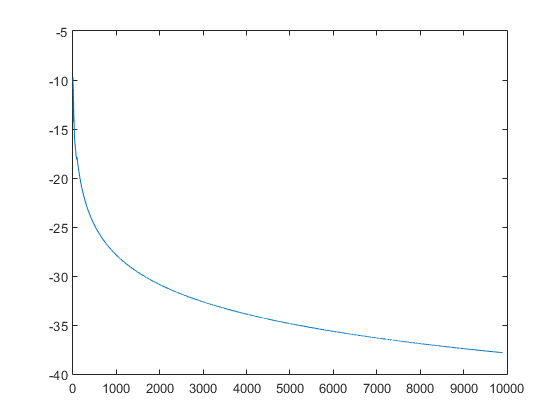
\includegraphics[scale=0.25]{u002.png} 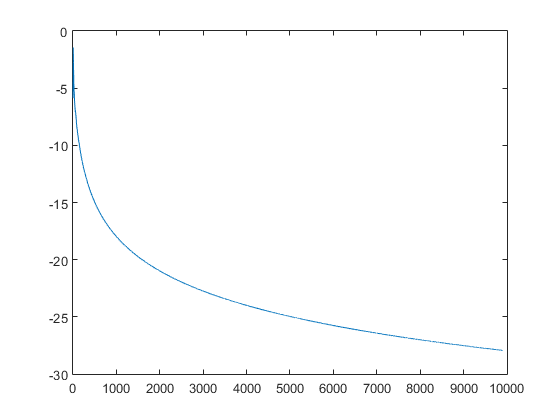
\includegraphics[scale=0.25]{u001.png} 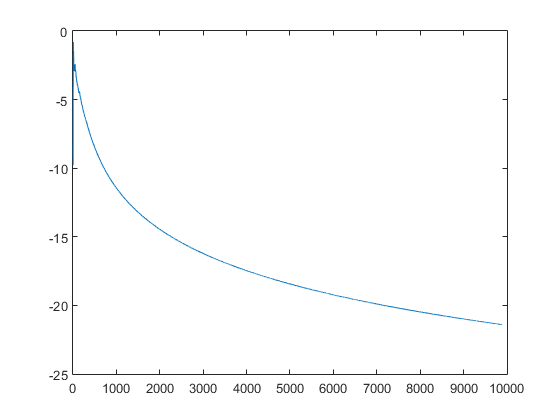
\includegraphics[scale=0.25]{u0005.png}
\end{figure}

On remarque que quand le steplength est grand, l'erreur quadratique moyenne converge plus vite et cela nous permet de gagner en nombre d'it\'eration et temps lors de l'ex\'ecution de l'algorithme. Par contre on ne peut pas choisir un $\mu$ trop grand non plus parce que \`a cause du fait de prendre $\mu$ trop grand, le residu va \^etre grand et donc l'erreur quadratique moyenne grand aussi. En fait, lors du choix du pas, on joue avec le compromis entre la transitoire et la fluctuation.
\paragraph{3.} On applique l'algorithme de LMS \`a l'annulation d'\'echo. On a les deux voies donn\'ees : y (le signal sortant du haut parleur) et z (le signal \`a l'entr\'ee du micro). Pour effectuer la m\'ethode de LMS, on peut prendre z au lieu de x en entr\'ee de la fonction LMS car ils ont la m\^eme esp\'erance. On \'estime le signal d'\'echo $\widehat{x}$ avec cette fonction et on fait sortir le signal am\'elior\'e (sans \'echo) qui est \'egal \`a la diff\'erence entre z et et $\widehat{x}$. On \'ecoute r\'espectivement le signal \`a l'ent\'ee du micro, le signal sans \'echo \`a la sortie et le signal d'\'echo estim\'e. On remarque qu'on n'arrive pas \`a enlever compl\`etement l'\'echo mais l'\'echo a \'et\'e bien r\'eduit gr\^ace \`a cet algorithme. Comme ce qu'on peut voir dans le graphe ci-dessous, les deux signaux plot\'es ont \`a peu pres la m\^eme forme mais si on constate que les parties ayant une amplitude plus faible repr\'esente l\'echo, le signal en sortie de l'algorithme a bien une amplitude quasiment nulle en ces parties. Cela v\'erifie le bon fonctionnement de l'algorithme.
\begin{center}
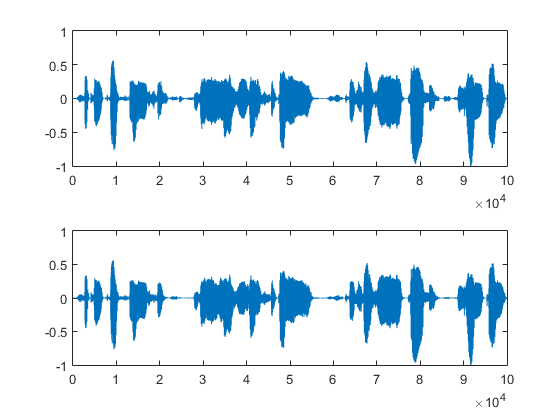
\includegraphics[scale=0.7]{result.png}
\end{center}

\end{document}